\newpage
    \section{Messwerte}
    Die folgenden Messwerte wurden uns zur Verfügung gestellt:
    \begin{table}
\centering
\caption{Messdaten}
\label{tab:mess}
\begin{tabular}{
    S[table-format=2.0]
    S[table-format=2.1]
    S[table-format=2.2]
    S[table-format=2.1]
    S[table-format=1.1]
    S[table-format=3.0]
}
\toprule
{$t \mathbin{/} \si{\minute} $} & {$T_1 \mathbin{/} \si{\celsius} $} 
    & {$p_1 \mathbin{/} \si{\bar} $} & {$T_2  \mathbin{/} \si{\celsius} $} 
    & {$p_2 \mathbin{/} \si{\bar} $} & {$N \mathbin{/} \si{\watt} $} \\

\midrule
0  & 21.7 &   4.0   &  21.7 &   4.1  &   120 \\
1  & 23.0 &   5.0   &  21.7 &   3.2  &   120 \\
2  & 24.3 &   5.5   &  21.6 &   3.4  &   120 \\
3  & 25.3 &   6.0   &  21.5 &   3.5  &   120 \\
4  & 26.4 &   6.0   &  20.8 &   3.5  &   120 \\
5  & 27.5 &   6.0   &  20.1 &   3.4  &   120 \\
6  & 28.8 &   6.5   &  19.2 &   3.3  &   120 \\
7  & 29.7 &   6.5   &  18.5 &   3.2  &   120 \\
8  & 30.9 &   7.0   &  17.7 &   3.2  &   120 \\
9  & 31.9 &   7.0   &  16.9 &   3.0  &   120 \\
10 & 32.9 &   7.0   &  16.2 &   3.0  &   120 \\
11 & 33.9 &   7.5   &  15.5 &   2.9  &   120 \\
12 & 34.8 &   7.5   &  14.9 &   2.8  &   120 \\
13 & 35.7 &   8.0   &  14.2 &   2.8  &   120 \\
14 & 36.7 &   8.0   &  13.6 &   2.7  &   120 \\
15 & 37.6 &   8.0   &  13.0 &   2.6  &   120 \\
16 & 38.4 &   8.5   &  12.4 &   2.6  &   120 \\
17 & 39.2 &   8.5   &  11.7 &   2.6  &   120 \\
18 & 40.0 &   9.0   &  11.3 &   2.5  &   120 \\
19 & 40.7 &   9.0   &  10.9 &   2.5  &   120 \\
20 & 41.4 &   9.0   &  10.4 &   2.4  &   120 \\
21 & 42.2 &   9.0   &  9.9  &   2.4  &   120 \\
22 & 42.9 &   9.5   &  9.5  &   2.4  &   120 \\
23 & 43.6 &   9.5   &  9.1  &   2.4  &   120 \\
24 & 44.3 &   10.0  &  8.7  &   2.4  &   120 \\
25 & 44.9 &   10.0  &  8.3  &   2.4  &   120 \\
26 & 45.5 &   10.0  &  8.0  &   2.3  &   120 \\
27 & 46.1 &   10.0  &  7.7  &   2.2  &   122 \\
28 & 46.7 &   10.5  &  7.4  &   2.2  &   122 \\
29 & 47.3 &   10.5  &  7.1  &   2.2  &   122 \\
30 & 47.8 &   10.75 &  6.8  &   2.2  &   122 \\
31 & 48.4 &   11.0  &  5.6  &   2.2  &   122 \\
32 & 48.9 &   11.0  &  4.3  &   2.2  &   122 \\
33 & 49.4 &   11.0  &  3.4  &   2.2  &   122 \\
34 & 49.9 &   11.0  &  3.0  &   2.2  &   122 \\
35 & 50.3 &   11.0  &  2.9  &   2.2  &   122 \\
\bottomrule
\end{tabular}

\end{table}

    %5
    \newpage
    \section{Auswertung}
        \subsection{Aufgabenteil a)}
        \begin{figure}
               \centering
               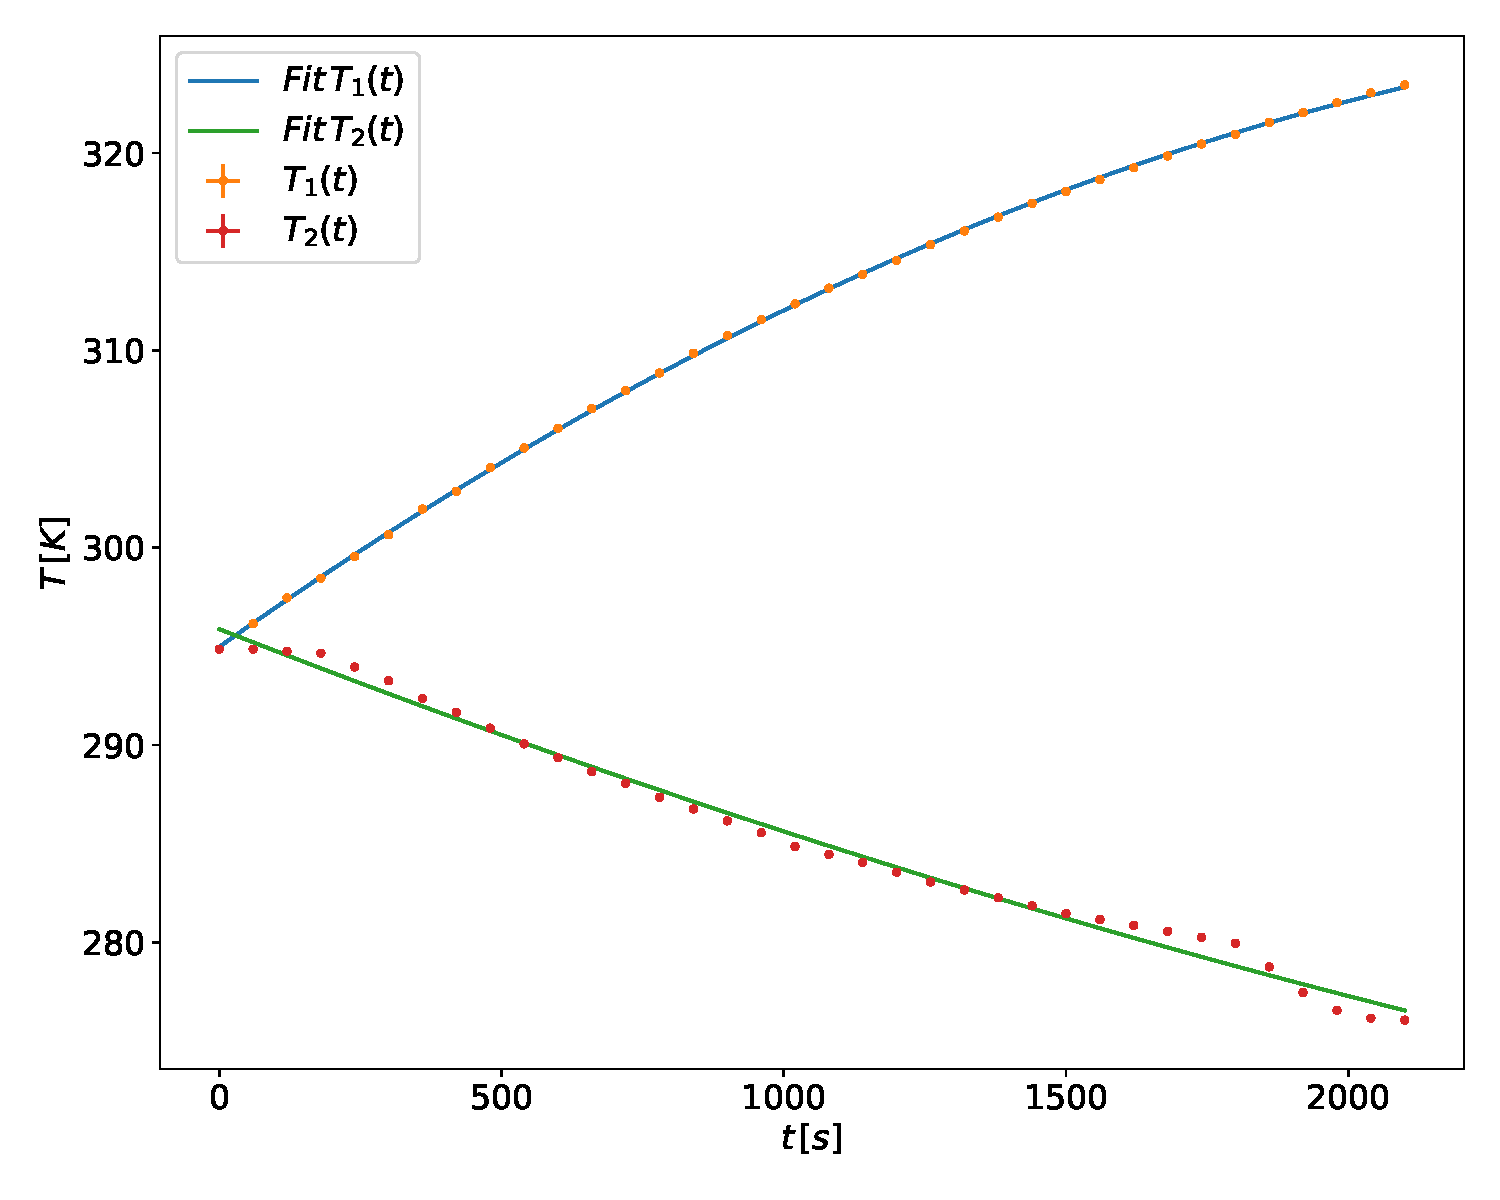
\includegraphics[width=\textwidth]{grafic.pdf}
               \caption{Auswertung mit ausgleichsgeraden}
               \label{fig:grafic}
        \end{figure}


            
        \newpage
        \subsection{Aufgabenteil b)}

        Eine nicht-lineare Ausgleichsrechnung der Temperaturverläufe mithilfe der Näherungsfunktion
        \begin{equation}
        T(t)=At^2 + Bt + C
        \end{equation}

        ergibt die folgenden Parameter:

        \begin{table}
        \centering
        \label{tab:parameterabc}
        \begin{tabular}{c c c c}
        \toprule
        $T$ & $A$ & $B$ & $C$ \\
        \midrule
        1 & -0.00000322 $\pm$ 0.00000004 & 0.02027984  $\pm$ 0.00009110 & 294.97008058 $\pm$ 0.04134538 \\
        2 & 0.00000096  $\pm$ 0.00000027 & -0.01120872 $\pm$ 0.00058032 & 295.87018724 $\pm$ 0.26336067 \\
        \bottomrule
        \end{tabular}
        \caption{Parameter für $T_1$ und $T_2$}
        \end{table}


        \subsection{Aufgabenteil c)}

        Im folgenden werden die Differentialquotienten $\frac{\symup{d} T_1}{\symup{d} t}$ und $\frac{\symup{d} T_2}{\symup{d} t}$ für vier verschiedene Temperaturen berechnet.
        Wir haben uns für die Temperaturen bei 8min, 16min, 24min und 32min entschieden.
        Es werden nun die entsprechenden Steigungen aus der Ableitung der Näherungsfunktion entnommen.

        \begin{equation}
        \frac{\symup{d}T}{\symup{d}t} = 2At + B
        \end{equation}

        Daraus ergeben sich folgende Steigungen:
        
        \begin{table}
        \centering
        \label{tab:differentialquotienten}
        \begin{tabular}{c c c}
        \toprule
        $t \mathbin{/} \si{\minute} $ & $\frac{\symup{d}T_1}{\symup{d}t} \mathbin{/} \si{\celsius}$ & $\frac{\symup{d}T_2}{\symup{d}t} \mathbin{/} \si{\celsius}$ \\
        \midrule
        8  & 0.01757091 $\pm$ 0.00012633 & -0.01040648 $\pm$ 0.00012633 \\
        16 & 0.01447498 $\pm$ 0.00016659 & -0.00948964 $\pm$ 0.00016659 \\
        24 & 0.01137906 $\pm$ 0.00020684 & -0.00857280 $\pm$ 0.00020684 \\
        32 & 0.00828314 $\pm$ 0.00024710 & -0.00765597 $\pm$ 0.00024710 \\
        \bottomrule
        \end{tabular}
        \caption{Differentialquotienten für $T_1$ und $T_2$}
        \end{table}


        \newpage
        \subsection{Aufgabenteil d)}

        Nun soll die reale Güteziffer $\upsilon_\text{real}$ nach Gleichung (\ref{eqn:gueteziffer3}) und die theoretische Güteziffer $\upsilon_\text{theorie}$ nach Gleichung (\ref{eqn:Gueteziffer}) berechnet werden.

        \begin{table}
        \centering
        \label{tab:gueteziffer}
        \begin{tabular}{c c c}
        \toprule
        $t \mathbin{/} \si{\minute} $ & $\upsilon_\text{real}$ & $\upsilon_\text{theorie}$ \\
        \midrule
        8  & 2.503 $\pm$ 0.019 & 23.0341 $\pm$ 0.0076 \\
        16 & 2.052 $\pm$ 0.025 & 11.9827 $\pm$ 0.0038 \\
        24 & 1.601 $\pm$ 0.031 & 8.9171  $\pm$ 0.0028 \\
        32 & 1.13 $\pm$ 0.04 & 7.2209  $\pm$ 0.0022 \\
        \bottomrule
        \end{tabular}
        \caption{Bestimmung der Güteziffer}
        \end{table}



        \subsection{Aufgabenteil e)}


        \subsection{Aufgabenteil f)}

        $N_\text{mech}$ lässt sich nach Gleichung (\ref{eqn:nmech2}) bestimmen.
        $\kappa$ beträgt in diesem Fall 1.14

        \begin{table}
        \centering
        \label{tab:kompressorleistung}
        \begin{tabular}{c c}
        \toprule
        $t \mathbin{/} \si{\minute} $ & $N_\text{mech} \mathbin{/} \si{\watt}$ & $\frac{\symup{d}T_2}{\symup{d}t} \mathbin{/} \si{\celsius}$ \\
        \midrule
        8  & 0.01757091 $\pm$ 0.00012633 \\
        16 & 0.01447498 $\pm$ 0.00016659 \\
        24 & 0.01137906 $\pm$ 0.00020684 \\
        32 & 0.00828314 $\pm$ 0.00024710 \\
        \bottomrule
        \end{tabular}
        \caption{Bestimmung der mechanischen Kompressorleistung}
        \end{table}

        